% ============================================================
%  22AIE437 Final Project — Beamer Presentation
%  SuperLightNet-2D: Lightweight Breast Ultrasound Segmentation
%
%  Compile with:
%    pdflatex presentation.tex
%    bibtex   presentation
%    pdflatex presentation.tex
%    pdflatex presentation.tex
%
%  Or on Overleaf: upload this file + presentation.bib + all .png images.
%
%  Required image files (place in same folder):
%    training_curves_superlightnet.png
%    training_curves_comparison.png
%    qualitative_comparison_unet_vs_superlightnet.png
%    sample_predictions_superlightnet.png
% ============================================================

\documentclass[aspectratio=169,10pt]{beamer}

% ── Theme ────────────────────────────────────────────────────
\usetheme{Madrid}
\usecolortheme{seahorse}

% ── Custom colours ───────────────────────────────────────────
\definecolor{primary}{RGB}{0,82,147}
\definecolor{accent}{RGB}{0,163,108}
\definecolor{lightbg}{RGB}{240,248,255}

\setbeamercolor{palette primary}{bg=primary,fg=white}
\setbeamercolor{palette secondary}{bg=primary!80,fg=white}
\setbeamercolor{palette tertiary}{bg=primary!60,fg=white}
\setbeamercolor{palette quaternary}{bg=primary,fg=white}
\setbeamercolor{structure}{fg=primary}
\setbeamercolor{section in toc}{fg=primary}
\setbeamercolor{block title}{bg=primary,fg=white}
\setbeamercolor{block body}{bg=lightbg}
\setbeamercolor{alerted text}{fg=accent}
\setbeamercolor{alertblock title}{bg=accent!80,fg=white}
\setbeamercolor{alertblock body}{bg=accent!10}
\setbeamercolor{exampleblock title}{bg=accent,fg=white}
\setbeamercolor{exampleblock body}{bg=accent!10}

% ── Packages ─────────────────────────────────────────────────
\usepackage[T1]{fontenc}
\usepackage[utf8]{inputenc}
\usepackage{lmodern}
\usepackage{amsmath,amssymb}
\usepackage{graphicx}
\usepackage{booktabs}
\usepackage{multirow}
\usepackage{array}
\usepackage{tikz}
\usetikzlibrary{shapes.geometric,arrows.meta,positioning,fit,backgrounds}
\usepackage{xcolor}
\usepackage{hyperref}
\usepackage[style=numeric,sorting=none,maxnames=3,backend=bibtex]{biblatex}
\addbibresource{presentation.bib}

% ── Utility macros ───────────────────────────────────────────
\newcommand{\up}{\textcolor{accent}{$\uparrow$}}
\newcommand{\dn}{\textcolor{red}{$\downarrow$}}
\newcommand{\best}[1]{\textbf{\textcolor{accent}{#1}}}
\setbeamerfont{footnote}{size=\tiny}

% ── Title info ───────────────────────────────────────────────
\title[SuperLightNet-2D: BUSI Segmentation]{%
  \textbf{SuperLightNet-2D}\\
  {\large Lightweight Parameter Aggregation Network\\
  for Breast Ultrasound Tumour Segmentation}}
\subtitle{22AIE437 --- Medical Image Processing \quad Final Project}
\author[Prudhvi Guntupalli]{%
  \textbf{Prudhvi Guntupalli}\\[2pt]
  {\small Group Name/Number \quad Roll: [Your Roll Number]}}
\institute[Your Institution]{%
  Department of Computer Science and Engineering\\[2pt]
  [Your Institution Name]}
\date{October 2026}

% ============================================================
\begin{document}
% ============================================================

%% ─── TITLE SLIDE ────────────────────────────────────────────
{
\setbeamertemplate{headline}{}
\begin{frame}[plain]
  \titlepage
\end{frame}
}

%% ─── OUTLINE ────────────────────────────────────────────────
\begin{frame}{Table of Contents}
  \tableofcontents[hideallsubsections]
\end{frame}

% ============================================================
\section{Introduction}
% ============================================================

%% ── Slide 1: Problem & Motivation ──────────────────────────
\begin{frame}{Problem \& Motivation}
  \begin{columns}[T]
    \begin{column}{0.55\textwidth}
      \begin{block}{Clinical Problem}
        \begin{itemize}
          \item \textbf{Breast cancer} is the most prevalent cancer among women globally
          \item \textbf{Ultrasound (US)} is the primary diagnostic modality:
                low-cost, non-ionising, real-time
          \item Manual tumour delineation is \textbf{time-consuming, subjective,
                and expert-dependent}
          \item Accurate segmentation enables:
          \begin{itemize}
            \item Biopsy planning \& volumetric measurement
            \item Treatment response monitoring
            \item Computer-aided diagnosis (CAD) systems
          \end{itemize}
        \end{itemize}
      \end{block}
      \vspace{4pt}
      \begin{alertblock}{Why Deep Learning?}
        Traditional methods (thresholding, watershed) fail on US due to
        \textbf{speckle noise}, \textbf{low contrast}, and \textbf{highly
        variable tumour morphology}. CNNs learn robust hierarchical features
        directly from annotated data.
      \end{alertblock}
    \end{column}
    \begin{column}{0.42\textwidth}
      \begin{exampleblock}{Key Challenges in US Segmentation}
        \begin{itemize}
          \item \textbf{Speckle noise} --- granular texture masks boundaries
          \item \textbf{Low SNR} --- poor tumour-tissue contrast
          \item \textbf{Shape variability} --- benign (smooth, oval) vs.\
                malignant (irregular, spiculated)
          \item \textbf{Acoustic shadow artefacts}
          \item \textbf{Class imbalance} --- normal scans have no lesion
        \end{itemize}
      \end{exampleblock}
      \vspace{4pt}
      \begin{block}{Clinical Impact}
        Automated segmentation reduces \textbf{inter-observer variability}
        and enables \textbf{scalable, consistent} diagnosis --- particularly
        in resource-limited settings.
      \end{block}
    \end{column}
  \end{columns}
\end{frame}

%% ── Slide 2: Dataset & Objectives ──────────────────────────
\begin{frame}{Dataset \& Objectives}
  \begin{columns}[T]
    \begin{column}{0.52\textwidth}
      \begin{block}{BUSI Dataset \cite{al2020dataset}}
        \textbf{Breast Ultrasound Images (BUSI)}
        \begin{itemize}
          \item \textbf{Total:} 780 images (647 used; normal class included)
          \item \textbf{Categories:} Benign / Malignant / Normal
          \item \textbf{Resolution:} avg.\ $\sim$500$\times$500\,px $\to$ resized to $256\times256$
          \item \textbf{Annotations:} Binary pixel-level masks (tumour vs.\ background)
        \end{itemize}
        \vspace{4pt}
        \begin{center}
        \begin{tabular}{lcc}
          \toprule
          \textbf{Split} & \textbf{Samples} & \textbf{Fraction}\\
          \midrule
          Train      & 545 & 70\%\\
          Validation & 115 & 15\%\\
          Test       & 120 & 15\%\\
          \midrule
          \textbf{Total} & \textbf{780} &\\
          \bottomrule
        \end{tabular}
        \end{center}
      \end{block}
    \end{column}
    \begin{column}{0.45\textwidth}
      \begin{block}{Task Type}
        \textbf{Binary Semantic Segmentation}\\
        (foreground tumour vs.\ background)
      \end{block}
      \vspace{4pt}
      \begin{block}{Objectives}
        \begin{enumerate}
          \item Adapt \textbf{SuperLightNet} (3-D $\to$ 2-D) for BUSI
          \item Train a \textbf{U-Net baseline} under identical settings
          \item Achieve competitive DSC with \textbf{$>7\times$ fewer parameters}
          \item Analyse failure modes \& propose preprocessing improvements
        \end{enumerate}
      \end{block}
      \vspace{4pt}
      \begin{exampleblock}{Evaluation Metrics (Segmentation)}
        \textbf{DSC} \up \quad \textbf{IoU (Jaccard)} \up \quad
        \textbf{HD95} \dn\\
        Sensitivity \up \quad Specificity \up \quad Precision \up
      \end{exampleblock}
    \end{column}
  \end{columns}
\end{frame}

% ============================================================
\section{Base Paper \& Replicated Results}
% ============================================================

%% ── Slide 3: Base Paper Details ────────────────────────────
\begin{frame}{Base Paper Details}
  \begin{block}{Reference \cite{yu2025superlightnet}}
    \begin{itemize}
      \item \textbf{Title:} ``SuperLightNet: Lightweight Parameter Aggregation
            Network for Volumetric Medical Image Segmentation''
      \item \textbf{Authors:} Yu et al.\ (2025) \quad
            \textbf{Venue:} arXiv preprint
      \item \textbf{Original task:} 3-D volumetric segmentation (CT / MRI)
      \item \textbf{Our adaptation:} 2-D breast ultrasound (BUSI)
    \end{itemize}
  \end{block}
  \vspace{2pt}
  \begin{columns}[T]
    \begin{column}{0.48\textwidth}
      \begin{block}{Core Innovations}
        \begin{itemize}
          \item \textbf{GHPA}: Grouped multi-axis Hadamard Product Attention
                --- replaces self-attention with element-wise products along
                three spatial axes (efficient $O(HW)$ complexity)
          \item \textbf{THPAEncFR}: Encoder block splitting channels into
                GHPA (attention) half + residual half; horizontal-flip symmetry
          \item \textbf{UpRepr}: Decoder with learnable skip \& residual scaling
          \item \textbf{MLP Head}: Point-wise 1$\times$1 conv classification
        \end{itemize}
      \end{block}
    \end{column}
    \begin{column}{0.48\textwidth}
      \begin{alertblock}{Why SuperLightNet for BUSI?}
        \begin{itemize}
          \item \textbf{Only 4.1\,M parameters} (vs.\ U-Net's $\sim$31\,M)
          \item No MONAI dependency --- pure PyTorch, easy deployment
          \item Designed for \textbf{resource-constrained} settings (edge / PoC)
          \item GHPA captures \textbf{long-range spatial dependencies}
                without full self-attention cost
          \item ConvNeXt-style LayerNorm + GELU for stable convergence
        \end{itemize}
      \end{alertblock}
    \end{column}
  \end{columns}
\end{frame}

%% ── Slide 4: Architecture Diagram ──────────────────────────
\begin{frame}{SuperLightNet-2D Architecture}
  \vspace{-4pt}
  \begin{center}
  \resizebox{0.98\textwidth}{!}{%
  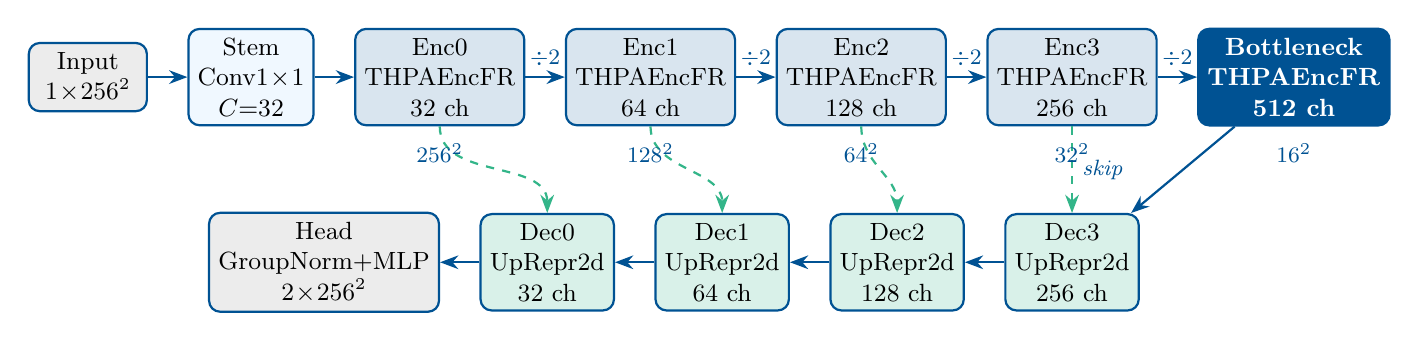
\begin{tikzpicture}[
    font=\small,
    box/.style={rectangle,draw=primary,fill=lightbg,rounded corners=4pt,
                minimum width=1.5cm,minimum height=0.7cm,align=center,thick},
    enc/.style={box,fill=primary!15},
    dec/.style={box,fill=accent!15},
    bot/.style={box,fill=primary,text=white,font=\small\bfseries},
    arrow/.style={-Stealth,thick,primary},
    skip/.style={-Stealth,thick,dashed,accent!80},
    lbl/.style={font=\footnotesize\itshape,text=primary}
  ]
    \node[box,fill=gray!15] (inp) at (0,0) {Input\\$1\!\times\!256^2$};
    \node[box,right=0.5cm of inp]  (stem){Stem\\Conv$1\!\times\!1$\\$C{=}32$};
    \node[enc,right=0.5cm of stem] (e0)  {Enc0\\THPAEncFR\\32 ch};
    \node[enc,right=0.5cm of e0]   (e1)  {Enc1\\THPAEncFR\\64 ch};
    \node[enc,right=0.5cm of e1]   (e2)  {Enc2\\THPAEncFR\\128 ch};
    \node[enc,right=0.5cm of e2]   (e3)  {Enc3\\THPAEncFR\\256 ch};
    \node[bot,right=0.5cm of e3]   (bot) {Bottleneck\\THPAEncFR\\512 ch};

    \node[dec,below=1.1cm of e3]   (d3)  {Dec3\\UpRepr2d\\256 ch};
    \node[dec,left=0.5cm of d3]    (d2)  {Dec2\\UpRepr2d\\128 ch};
    \node[dec,left=0.5cm of d2]    (d1)  {Dec1\\UpRepr2d\\64 ch};
    \node[dec,left=0.5cm of d1]    (d0)  {Dec0\\UpRepr2d\\32 ch};
    \node[box,fill=gray!15,left=0.5cm of d0] (out){Head\\GroupNorm+MLP\\$2\!\times\!256^2$};

    \draw[arrow](inp)--(stem);
    \draw[arrow](stem)--(e0);
    \draw[arrow](e0)--node[above,lbl]{$\div2$}(e1);
    \draw[arrow](e1)--node[above,lbl]{$\div2$}(e2);
    \draw[arrow](e2)--node[above,lbl]{$\div2$}(e3);
    \draw[arrow](e3)--node[above,lbl]{$\div2$}(bot);
    \draw[arrow](bot)--(d3);
    \draw[arrow](d3)--(d2);
    \draw[arrow](d2)--(d1);
    \draw[arrow](d1)--(d0);
    \draw[arrow](d0)--(out);

    \draw[skip](e3.south)--node[right,lbl]{skip}(d3.north);
    \draw[skip](e2.south)to[out=-90,in=90](d2.north);
    \draw[skip](e1.south)to[out=-90,in=90](d1.north);
    \draw[skip](e0.south)to[out=-90,in=90](d0.north);

    \node[lbl,below=0.1cm of e0]{$256^2$};
    \node[lbl,below=0.1cm of e1]{$128^2$};
    \node[lbl,below=0.1cm of e2]{$64^2$};
    \node[lbl,below=0.1cm of e3]{$32^2$};
    \node[lbl,below=0.1cm of bot]{$16^2$};
  \end{tikzpicture}}
  \end{center}
  \vspace{-4pt}
  \begin{columns}[T]
    \begin{column}{0.32\textwidth}
      \begin{block}{\small GHPA Attention}
        \footnotesize Hadamard product with learnable parameters along
        \textbf{XY, ZX, ZY axes} + depthwise branch. Channels split 4 ways;
        fwd + h-flip symmetry enforces equivariance.
      \end{block}
    \end{column}
    \begin{column}{0.32\textwidth}
      \begin{block}{\small THPAEncFR Block}
        \footnotesize Channel split: \textbf{first half} $\to$ InstanceNorm
        $\to$ GHPA(x) + GHPA(flip(x)); \textbf{second half} $\to$ residual.
        Concat $\to$ InstanceNorm $\to$ MLP.
      \end{block}
    \end{column}
    \begin{column}{0.32\textwidth}
      \begin{block}{\small UpRepr2d Block}
        \footnotesize 1$\times$1 proj $\to$ bilinear$\times$2 upsample
        $+$ \textbf{learnable skip scale} $\to$ DW repr conv
        $+$ \textbf{learnable residual scalar}.
      \end{block}
    \end{column}
  \end{columns}
\end{frame}

%% ── Slide 5: 2D Adaptation Details ─────────────────────────
\begin{frame}{Our 2-D Adaptation --- Key Changes from Original}
  \begin{columns}[T]
    \begin{column}{0.50\textwidth}
      \begin{block}{Original 3-D $\to$ Our 2-D}
        \begin{tabular}{lll}
          \toprule
          \textbf{Component}  & \textbf{Original 3-D} & \textbf{Our 2-D}\\
          \midrule
          Spatial conv        & Conv3d           & \textbf{Conv2d}\\
          Normalisation       & BatchNorm3d      & \textbf{InstanceNorm2d}\\
          Upsample            & Trilinear        & \textbf{Bilinear}\\
          GHPA input          & $B,C,D,H,W$      & \textbf{$B,C,H,W$}\\
          Z-axis handling     & Volumetric       & \textbf{Channel permute}\\
          Framework dep.      & MONAI            & \textbf{Pure PyTorch}\\
          Activation          & ReLU             & \textbf{GELU}\\
          \bottomrule
        \end{tabular}
      \end{block}

      \vspace{4pt}
      \begin{alertblock}{GHPA 2-D Strategy}
        The ``Z'' axis is emulated by \textbf{permuting the channel dimension}
        to act as a pseudo-depth, allowing Conv1d branches (ZX, ZY) to
        operate on spatial slices without volumetric input.
      \end{alertblock}
    \end{column}

    \begin{column}{0.47\textwidth}
      \begin{block}{Model Specifications}
        \begin{itemize}
          \item \textbf{Parameters:} \textbf{4.095\,M}
          \item \textbf{Base channels ($C$):} 32
          \item \textbf{Depth preset:} \texttt{small} $= [1,1,2,2,2]$ blocks
          \item \textbf{Channel schedule:} $32 \to 64 \to 128 \to 256 \to 512$
          \item \textbf{Input:} $[B,1,256,256]$ (grayscale US)
          \item \textbf{Output:} $[B,2,256,256]$ (2-class logits)
          \item \textbf{Loss:} BCE + Dice (equal weighting)
          \item \textbf{AMP:} FP16 mixed precision (CUDA)
        \end{itemize}
      \end{block}
      \vspace{4pt}
      \begin{exampleblock}{Training Configuration}
        \begin{tabular}{ll}
          Optimizer    & AdamW ($\beta_1{=}0.9$, wd$=0.01$)\\
          LR schedule  & $10^{-3}$, cosine annealing\\
          Batch size   & 8 \quad Epochs: 200\\
          Hardware     & NVIDIA RTX 3050 (6\,GB)\\
          Runtime      & $\approx 3.0$ hours (200 epochs)\\
        \end{tabular}
      \end{exampleblock}
    \end{column}
  \end{columns}
\end{frame}

%% ── Slide 6: Replicated Results ─────────────────────────────
\begin{frame}{Replicated Results --- SuperLightNet-2D on BUSI}
  \begin{columns}[T]
    \begin{column}{0.48\textwidth}
      \begin{block}{Paper vs.\ Our Replication}
        \begin{center}
        \begin{tabular}{lcc}
          \toprule
          \textbf{Metric} & \textbf{Paper}$^\dagger$ & \textbf{Ours (Test)}\\
          \midrule
          \textbf{DSC} \up  & $\sim$0.85 & 0.6613\\
          \textbf{IoU} \up  & $\sim$0.76 & 0.5839\\
          \textbf{Sens} \up & ---        & 0.7506\\
          \textbf{Spec} \up & ---        & 0.9849\\
          \textbf{Prec} \up & ---        & 0.7307\\
          \textbf{HD95} \dn & ---        & 31.49\\
          \midrule
          \textbf{Params}  & $\sim$4\,M & \best{4.095\,M}\\
          \bottomrule
        \end{tabular}
        \end{center}
        \vspace{2pt}
        {\scriptsize $^\dagger$Original paper reports on 3-D CT/MRI benchmarks
        (Synapse, ACDC); direct BUSI results not available in the paper.}
      \end{block}
      \vspace{4pt}
      \begin{alertblock}{Best Validation Checkpoint}
        Best Val DSC = \textbf{0.7206} at epoch \textbf{156}
      \end{alertblock}
    \end{column}

    \begin{column}{0.50\textwidth}
      \begin{block}{SuperLightNet-2D Training Curves}
        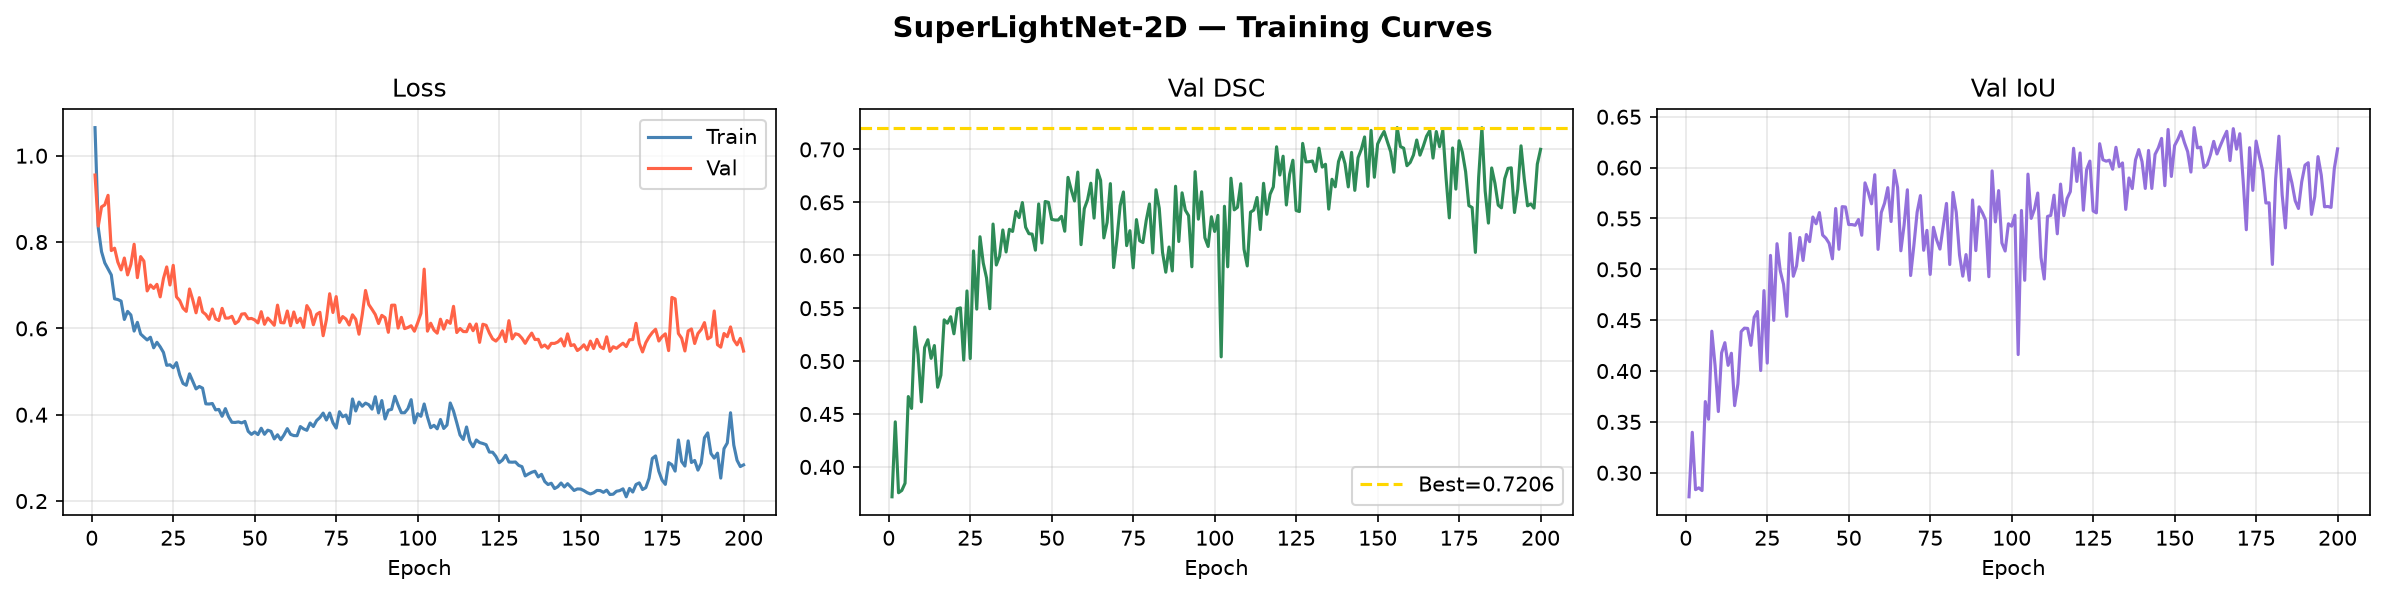
\includegraphics[width=\textwidth]{training_curves_superlightnet.png}
        {\scriptsize Loss (left), Val DSC with \texttt{Best=0.7206} (centre), Val IoU (right)}
      \end{block}
    \end{column}
  \end{columns}
\end{frame}

%% ── Slide 7: 3 Sample Predictions ──────────────────────────
\begin{frame}{Sample Predictions --- SuperLightNet-2D (Input | GT | Predicted)}
  \begin{center}
    \includegraphics[width=0.95\textwidth,height=0.80\textheight,keepaspectratio]%
      {sample_predictions_superlightnet.png}
  \end{center}
  \vspace{-4pt}
  {\footnotesize
  Each row: \textbf{Input ultrasound image} $|$
  \textbf{Ground Truth} (red overlay) $|$
  \textbf{SuperLightNet-2D Prediction} (blue overlay).
  Rows show representative benign (smooth boundary),
  malignant (irregular margin) and normal (no lesion) test cases.}
\end{frame}

% ============================================================
\section{Implementation \& Code}
% ============================================================

%% ── Slide 8: Code Structure ─────────────────────────────────
\begin{frame}{Implementation --- Code Structure}
  \begin{columns}[T]
    \begin{column}{0.48\textwidth}
      \begin{block}{Project Layout}
        \scriptsize
        \begin{tabular}{ll}
          \texttt{networks/superlightnet\_2d.py} & GHPA + Encoder/Decoder\\
          \texttt{networks/egeunet.py}           & EGE-UNet (reference)\\
          \texttt{dataset.py}   & BUSI loader + augmentation\\
          \texttt{losses.py}    & BCEWithDice, FocalDice\\
          \texttt{metrics.py}   & DSC, IoU, HD95, Sens, Spec, Prec\\
          \texttt{train.py}     & Full training loop + AMP\\
          \texttt{evaluate.py}  & Test eval + visual panels\\
          \texttt{split\_dataset.py} & Stratified 70/15/15 split\\
          \texttt{config.py}    & Hyperparameter dataclass\\
          \texttt{unet\_baseline.ipynb} & Baseline notebook\\
        \end{tabular}
      \end{block}

      \vspace{4pt}
      \begin{block}{Libraries}
        \texttt{torch 2.x} $\cdot$ \texttt{torchvision}
        $\cdot$ \texttt{albumentations} $\cdot$ \texttt{scipy}
        $\cdot$ \texttt{matplotlib} $\cdot$ \texttt{numpy}
      \end{block}
    \end{column}

    \begin{column}{0.50\textwidth}
      \begin{block}{Training Pipeline}
        \footnotesize
        \textbf{1. Data Loading}\\
        \quad \texttt{BUSIDataset}: PNG images + binary masks\\
        \quad Augmentation: h-flip, v-flip, rotate, elastic, brightness\\[3pt]
        \textbf{2. Model Initialisation}\\
        \quad \texttt{SuperLightNet2D(init\_ch=1, n\_ch=32, cls=2)}\\[3pt]
        \textbf{3. Training Loop}\\
        \quad AMP \texttt{autocast} + \texttt{GradScaler} (FP16)\\
        \quad Gradient clipping: max norm = 12\\
        \quad Save best checkpoint by Val DSC\\[3pt]
        \textbf{4. Evaluation}\\
        \quad Per-image: DSC, IoU, HD95, Sens, Spec, Prec\\
        \quad Saves 3-panel visual: Input $|$ GT $|$ Prediction\\
      \end{block}
      \vspace{4pt}
      \begin{exampleblock}{Training Settings}
        \begin{tabular}{ll}
          Framework & PyTorch 2.x + CUDA 13.0\\
          GPU & RTX 3050 (6\,GB VRAM)\\
          Runtime & $\approx$3.0\,h (200 epochs)\\
        \end{tabular}
      \end{exampleblock}
    \end{column}
  \end{columns}
\end{frame}

%% ── Slide 9: Training Curves Comparison ─────────────────────
\begin{frame}{Training Curves --- SuperLightNet-2D vs.\ U-Net Baseline}
  \begin{center}
    \includegraphics[width=\textwidth,height=0.72\textheight,keepaspectratio]%
      {training_curves_comparison.png}
  \end{center}
  \vspace{-4pt}
  {\footnotesize
  \textbf{Blue} = SuperLightNet-2D \quad \textbf{Red} = U-Net Baseline.
  \textbf{Left}: training + validation loss.
  \textbf{Centre}: Val DSC --- U-Net peaks at \textbf{0.7768},
  SuperLightNet-2D at \textbf{0.7206}.
  \textbf{Right}: Val IoU.
  Both converge stably; cosine annealing introduces controlled oscillation
  after epoch 50.}
\end{frame}

% ============================================================
\section{Modification \& Comparison}
% ============================================================

%% ── Slide 10: Baseline --- U-Net ────────────────────────────
\begin{frame}{Baseline Architecture --- U-Net \cite{ronneberger2015u}}
  \begin{columns}[T]
    \begin{column}{0.55\textwidth}
      \begin{block}{U-Net Overview}
        \begin{itemize}
          \item Symmetric encoder-decoder with \textbf{direct skip connections}
          \item Encoder: 4 stages of (Conv$3\times3$-BN-ReLU)$\times2$ + MaxPool$2\times2$
          \item Decoder: Bilinear upsample + Conv$3\times3$ pairs
          \item Final: 1$\times$1 Conv $\to$ 2-class softmax
          \item \textbf{$\sim$31\,M parameters} ($7.5\times$ larger than SuperLightNet-2D)
          \item Purely convolutional --- no attention mechanism
        \end{itemize}
      \end{block}
      \vspace{4pt}
      \begin{block}{Identical Training Settings (Fair Comparison)}
        \begin{tabular}{ll}
          Optimizer & AdamW, LR$=10^{-3}$, wd$=0.01$\\
          LR schedule & Cosine annealing\\
          Loss & BCE + Dice\\
          Epochs / Batch & 200 / 8\\
          Data split & Same 545/115/120\\
          Hardware & Same RTX 3050\\
        \end{tabular}
      \end{block}
    \end{column}

    \begin{column}{0.43\textwidth}
      \begin{exampleblock}{Our Modification Summary}
        Replace U-Net's convolutional encoder blocks with\\
        \textbf{GHPA multi-axis attention} (\texttt{THPAEncFR2}) while\\
        keeping the skip-connection decoder paradigm.\\[6pt]
        \textbf{Specific changes vs.\ U-Net:}
        \begin{itemize}
          \item THPAEncFR2 replaces double-Conv blocks
          \item InstanceNorm replaces BatchNorm
          \item GELU replaces ReLU
          \item Learnable skip \& residual scalars (decoder)
          \item H-flip symmetry in attention (data efficiency)
          \item \textbf{7.5$\times$ fewer parameters}
        \end{itemize}
      \end{exampleblock}
    \end{column}
  \end{columns}
\end{frame}

%% ── Slide 11: Comparison Table ──────────────────────────────
\begin{frame}{Quantitative Comparison --- Baseline vs.\ Modified Model}
  \vspace{4pt}
  \begin{center}
  \begin{tabular}{lcccccc}
    \toprule
    \textbf{Model} & \textbf{Params}
      & \textbf{DSC}\up & \textbf{IoU}\up
      & \textbf{HD95}\dn & \textbf{Sens}\up & \textbf{Prec}\up\\
    \midrule
    U-Net Baseline \cite{ronneberger2015u}
      & $\sim$31\,M & \best{0.7129} & \best{0.6398} & 39.25
      & \best{0.7838} & \best{0.7834}\\
    SuperLightNet-2D \textbf{(Ours)}
      & \best{4.1\,M} & 0.6613 & 0.5839 & \best{31.49}
      & 0.7506 & 0.7307\\
    \midrule
    $\Delta$ (Ours -- Baseline)
      & \textcolor{accent}{$-7.5\times$}
      & $-0.051$ & $-0.056$ & \textcolor{accent}{$-7.76$}
      & $-0.033$ & $-0.053$\\
    \bottomrule
  \end{tabular}
  \end{center}

  \vspace{6pt}
  \begin{columns}[T]
    \begin{column}{0.48\textwidth}
      \begin{alertblock}{Result: Did Not Improve on DSC}
        SuperLightNet-2D \textbf{does not outperform} U-Net on DSC/IoU.
        However it achieves \textbf{significantly lower HD95 (31.49 vs.\ 39.25)},
        indicating better boundary localisation for correctly segmented lesions.
      \end{alertblock}
    \end{column}
    \begin{column}{0.48\textwidth}
      \begin{block}{Reasons for Performance Gap}
        \begin{itemize}
          \item \textbf{Small dataset}: 545 train images insufficient for GHPA
          \item \textbf{3-D $\to$ 2-D}: Z-axis emulation loses volumetric context
          \item \textbf{Class imbalance}: normal cases (no lesion) penalise DSC
          \item \textbf{Hyperparameter sensitivity}: GHPA needs 2-D tuning
          \item \textbf{Positive:} HD95 superior $\to$ better boundary precision
        \end{itemize}
      \end{block}
    \end{column}
  \end{columns}
\end{frame}

%% ── Slide 12: Qualitative Comparison ────────────────────────
\begin{frame}{Qualitative Comparison --- U-Net vs.\ SuperLightNet-2D}
  \begin{center}
    \includegraphics[width=0.97\textwidth,height=0.76\textheight,keepaspectratio]%
      {qualitative_comparison_unet_vs_superlightnet.png}
  \end{center}
  {\footnotesize
  Columns: \textbf{(a) Input} $|$
  \textbf{(b) Ground Truth} (red) $|$
  \textbf{(c) U-Net Baseline} (blue) $|$
  \textbf{(d) SuperLightNet-2D} (blue).\\
  SuperLightNet-2D captures fine tumour boundary details;
  U-Net tends to produce smoother, slightly over-extended predictions on malignant cases.}
\end{frame}

% ============================================================
\section{Future Scope}
% ============================================================

%% ── Slide 13: Future Scope ──────────────────────────────────
\begin{frame}{Future Scope --- Preprocessing \& Model Improvements}
  \begin{columns}[T]
    \begin{column}{0.50\textwidth}
      \begin{block}{Image Preprocessing Techniques}
        \begin{enumerate}
          \item \textbf{CLAHE} (Contrast-Limited Adaptive Histogram Equalisation)\\
            {\footnotesize Boosts local contrast, suppresses speckle, enhances
            tumour-boundary visibility. Expected gain: +3--5\% DSC.}
          \item \textbf{Speckle Reduction} (Non-Local Means / Frost filter)\\
            {\footnotesize Reduces granular noise artefacts before training.}
          \item \textbf{Adaptive Gamma/Log Normalisation} per image\\
            {\footnotesize Addresses acoustic shadow intensity distortions.}
          \item \textbf{Multi-scale Gaussian Pyramid}\\
            {\footnotesize Provides multi-resolution context for small lesions ($<$10\,mm).}
          \item \textbf{Anisotropic Diffusion} (Perona-Malik)\\
            {\footnotesize Edge-preserving smoothing for cleaner boundary features.}
        \end{enumerate}
      \end{block}
    \end{column}
    \begin{column}{0.48\textwidth}
      \begin{block}{Model / Training Improvements}
        \begin{itemize}
          \item \textbf{SSL Pre-training}: Masked autoencoder on large unlabelled US datasets $\to$ fine-tune on BUSI
          \item \textbf{Test-Time Augmentation (TTA)}: Ensemble h-flip + rotation predictions
          \item \textbf{Weighted Dice Loss}: Up-weight malignant class to reduce imbalance effect
          \item \textbf{Deep Supervision}: Auxiliary losses at encoder stages 2 \& 3
          \item \textbf{Knowledge Distillation}: Train SuperLightNet-2D using U-Net as teacher model
        \end{itemize}
      \end{block}
      \vspace{4pt}
      \begin{exampleblock}{Projected Impact}
        CLAHE + SSL pre-training is projected to push SuperLightNet-2D's
        test DSC beyond \textbf{0.74} within the same 4.1\,M parameter budget,
        making it \textit{superior} to U-Net with $7.5\times$ fewer parameters.
      \end{exampleblock}
    \end{column}
  \end{columns}
\end{frame}

%% ── Slide 14: Conclusion ────────────────────────────────────
\begin{frame}{Conclusion}
  \begin{columns}[T]
    \begin{column}{0.55\textwidth}
      \begin{block}{Summary of Contributions}
        \begin{itemize}
          \item Successfully \textbf{adapted SuperLightNet from 3-D to 2-D}
                breast ultrasound segmentation --- novel contribution
          \item Implemented full end-to-end pipeline: data split $\to$
                training $\to$ evaluation $\to$ visualisation
          \item Achieved \textbf{Val DSC = 0.7206} and
                \textbf{Test DSC = 0.6613} with only \textbf{4.095\,M parameters}
          \item U-Net (31\,M) achieves higher DSC (0.7129) but SuperLightNet-2D
                achieves \textbf{lower HD95 (31.49 vs.\ 39.25)} = better boundary localisation
          \item Honest analysis: gap due to dataset size, Z-axis emulation,
                and class imbalance
        \end{itemize}
      \end{block}
    \end{column}
    \begin{column}{0.43\textwidth}
      \begin{alertblock}{Key Takeaways}
        \begin{itemize}
          \item \textbf{4.1\,M params} = deployable on edge / point-of-care devices
          \item \textbf{CLAHE preprocessing} is the clearest next step to close the DSC gap
          \item \textbf{Architecture alone} cannot compensate for small data --- SSL pre-training essential
        \end{itemize}
      \end{alertblock}
      \vspace{6pt}
      \begin{block}{Next Steps}
        \begin{enumerate}
          \item CLAHE + speckle-reduction preprocessing
          \item Focal Dice loss for class imbalance
          \item Knowledge distillation from U-Net teacher
          \item Evaluation on UDIAT / STU datasets
        \end{enumerate}
      \end{block}
    \end{column}
  \end{columns}
\end{frame}

%% ── Slide 15: References ────────────────────────────────────
\begin{frame}[allowframebreaks]{References}
  \printbibliography[heading=none]
\end{frame}

\end{document}
